% Generated by Sphinx.
\def\sphinxdocclass{report}
\documentclass[letterpaper,10pt]{sphinxmanual}
\usepackage[utf8]{inputenc}
\DeclareUnicodeCharacter{00A0}{\nobreakspace}
\usepackage[T1]{fontenc}
\usepackage[english]{babel}
\usepackage{times}
\usepackage[Sonny]{fncychap}
\usepackage{longtable}
\usepackage{sphinx}
\usepackage{multirow}

% \pdfpagewidth 195mm
% \pdfpageheight 271mm
% \textwidth 6.0in
% \textheight 8.8in
% \oddsidemargin -0.1in
% \evensidemargin -0.1in

\textwidth 6.8in
\oddsidemargin -0.2in
\evensidemargin -0.3in

\usepackage{pdfpages}
\usepackage[BoldFont,CJKchecksingle]{xeCJK}
\usepackage{float}
\usepackage{ccaption}
\usepackage{pifont}
% \usepackage{fancybox}
\usepackage{fontspec,xunicode,xltxtra}

\setsansfont{DejaVu Serif}
% \setromanfont{DejaVu Sans Mono}
\setmainfont{DejaVu Serif}
\setmonofont{DejaVu Sans Mono}

% \setsansfont{WenQuanYi Micro Hei Light}
% \setromanfont{WenQuanYi Micro Hei Light}
% \setmainfont{WenQuanYi Micro Hei Light}
% \setmonofont{WenQuanYi Micro Hei Mono Light}
% STXihei
\setCJKsansfont[BoldFont={SimSun},ItalicFont={SimSun}]{SimSun}
\setCJKromanfont[BoldFont={SimSun},ItalicFont={SimSun}]{SimSun}
\setCJKmainfont[BoldFont={SimSun},ItalicFont={SimSun}]{SimSun}
\setCJKmonofont[BoldFont={SimSun},ItalicFont={SimSun}]{SimSun}

% \setCJKsansfont{Microsoft YaHei}
% \setCJKromanfont{Microsoft YaHei}
% \setCJKmainfont{Microsoft YaHei}
% \setCJKmonofont{Microsoft YaHei}

% \CJKaddspaces\CJKsetecglue{\hskip 0.15em plus 0.05em minus 0.05em}

\XeTeXlinebreaklocale "zh"
\XeTeXlinebreakskip = 0pt plus 1pt
\renewcommand{\baselinestretch}{1.3} 
\setcounter{tocdepth}{3}
\captiontitlefont{\small\sffamily}
\captiondelim{ - }
\renewcommand\today{\number\year年\number\month月\number\day日}      
\makeatletter
\renewcommand*\l@subsection{\@dottedtocline{2}{2.0em}{4.0em}}
\renewcommand*\l@subsubsection{\@dottedtocline{3}{3em}{5em}}
\makeatother
\titleformat{\chapter}[display]
{\bfseries\Huge}
{\filleft \Huge 第 \hspace{2 mm} \thechapter \hspace{4 mm} 章}
{4ex}
{\titlerule
\vspace{1ex}%
\filright}
[\vspace{1ex}%
\titlerule]
%\definecolor{VerbatimBorderColor}{rgb}{0.2,0.2,0.2}
\definecolor{VerbatimColor}{rgb}{0.95,0.95,0.95}


\title{用Sphinx写书}
\date{2013 年 06 月 18 日}
\release{1.0}
\author{HYRY Studio}
\newcommand{\sphinxlogo}{}
\renewcommand{\releasename}{发布}
\makeindex

\makeatletter
\def\PYG@reset{\let\PYG@it=\relax \let\PYG@bf=\relax%
    \let\PYG@ul=\relax \let\PYG@tc=\relax%
    \let\PYG@bc=\relax \let\PYG@ff=\relax}
\def\PYG@tok#1{\csname PYG@tok@#1\endcsname}
\def\PYG@toks#1+{\ifx\relax#1\empty\else%
    \PYG@tok{#1}\expandafter\PYG@toks\fi}
\def\PYG@do#1{\PYG@bc{\PYG@tc{\PYG@ul{%
    \PYG@it{\PYG@bf{\PYG@ff{#1}}}}}}}
\def\PYG#1#2{\PYG@reset\PYG@toks#1+\relax+\PYG@do{#2}}

\expandafter\def\csname PYG@tok@gd\endcsname{\def\PYG@tc##1{\textcolor[rgb]{0.63,0.00,0.00}{##1}}}
\expandafter\def\csname PYG@tok@gu\endcsname{\let\PYG@bf=\textbf\def\PYG@tc##1{\textcolor[rgb]{0.50,0.00,0.50}{##1}}}
\expandafter\def\csname PYG@tok@gt\endcsname{\def\PYG@tc##1{\textcolor[rgb]{0.00,0.27,0.87}{##1}}}
\expandafter\def\csname PYG@tok@gs\endcsname{\let\PYG@bf=\textbf}
\expandafter\def\csname PYG@tok@gr\endcsname{\def\PYG@tc##1{\textcolor[rgb]{1.00,0.00,0.00}{##1}}}
\expandafter\def\csname PYG@tok@cm\endcsname{\let\PYG@it=\textit\def\PYG@tc##1{\textcolor[rgb]{0.25,0.50,0.56}{##1}}}
\expandafter\def\csname PYG@tok@vg\endcsname{\def\PYG@tc##1{\textcolor[rgb]{0.73,0.38,0.84}{##1}}}
\expandafter\def\csname PYG@tok@m\endcsname{\def\PYG@tc##1{\textcolor[rgb]{0.13,0.50,0.31}{##1}}}
\expandafter\def\csname PYG@tok@mh\endcsname{\def\PYG@tc##1{\textcolor[rgb]{0.13,0.50,0.31}{##1}}}
\expandafter\def\csname PYG@tok@cs\endcsname{\def\PYG@tc##1{\textcolor[rgb]{0.25,0.50,0.56}{##1}}\def\PYG@bc##1{\setlength{\fboxsep}{0pt}\colorbox[rgb]{1.00,0.94,0.94}{\strut ##1}}}
\expandafter\def\csname PYG@tok@ge\endcsname{\let\PYG@it=\textit}
\expandafter\def\csname PYG@tok@vc\endcsname{\def\PYG@tc##1{\textcolor[rgb]{0.73,0.38,0.84}{##1}}}
\expandafter\def\csname PYG@tok@il\endcsname{\def\PYG@tc##1{\textcolor[rgb]{0.13,0.50,0.31}{##1}}}
\expandafter\def\csname PYG@tok@go\endcsname{\def\PYG@tc##1{\textcolor[rgb]{0.20,0.20,0.20}{##1}}}
\expandafter\def\csname PYG@tok@cp\endcsname{\def\PYG@tc##1{\textcolor[rgb]{0.00,0.44,0.13}{##1}}}
\expandafter\def\csname PYG@tok@gi\endcsname{\def\PYG@tc##1{\textcolor[rgb]{0.00,0.63,0.00}{##1}}}
\expandafter\def\csname PYG@tok@gh\endcsname{\let\PYG@bf=\textbf\def\PYG@tc##1{\textcolor[rgb]{0.00,0.00,0.50}{##1}}}
\expandafter\def\csname PYG@tok@ni\endcsname{\let\PYG@bf=\textbf\def\PYG@tc##1{\textcolor[rgb]{0.84,0.33,0.22}{##1}}}
\expandafter\def\csname PYG@tok@nl\endcsname{\let\PYG@bf=\textbf\def\PYG@tc##1{\textcolor[rgb]{0.00,0.13,0.44}{##1}}}
\expandafter\def\csname PYG@tok@nn\endcsname{\let\PYG@bf=\textbf\def\PYG@tc##1{\textcolor[rgb]{0.05,0.52,0.71}{##1}}}
\expandafter\def\csname PYG@tok@no\endcsname{\def\PYG@tc##1{\textcolor[rgb]{0.38,0.68,0.84}{##1}}}
\expandafter\def\csname PYG@tok@na\endcsname{\def\PYG@tc##1{\textcolor[rgb]{0.25,0.44,0.63}{##1}}}
\expandafter\def\csname PYG@tok@nb\endcsname{\def\PYG@tc##1{\textcolor[rgb]{0.00,0.44,0.13}{##1}}}
\expandafter\def\csname PYG@tok@nc\endcsname{\let\PYG@bf=\textbf\def\PYG@tc##1{\textcolor[rgb]{0.05,0.52,0.71}{##1}}}
\expandafter\def\csname PYG@tok@nd\endcsname{\let\PYG@bf=\textbf\def\PYG@tc##1{\textcolor[rgb]{0.33,0.33,0.33}{##1}}}
\expandafter\def\csname PYG@tok@ne\endcsname{\def\PYG@tc##1{\textcolor[rgb]{0.00,0.44,0.13}{##1}}}
\expandafter\def\csname PYG@tok@nf\endcsname{\def\PYG@tc##1{\textcolor[rgb]{0.02,0.16,0.49}{##1}}}
\expandafter\def\csname PYG@tok@si\endcsname{\let\PYG@it=\textit\def\PYG@tc##1{\textcolor[rgb]{0.44,0.63,0.82}{##1}}}
\expandafter\def\csname PYG@tok@s2\endcsname{\def\PYG@tc##1{\textcolor[rgb]{0.25,0.44,0.63}{##1}}}
\expandafter\def\csname PYG@tok@vi\endcsname{\def\PYG@tc##1{\textcolor[rgb]{0.73,0.38,0.84}{##1}}}
\expandafter\def\csname PYG@tok@nt\endcsname{\let\PYG@bf=\textbf\def\PYG@tc##1{\textcolor[rgb]{0.02,0.16,0.45}{##1}}}
\expandafter\def\csname PYG@tok@nv\endcsname{\def\PYG@tc##1{\textcolor[rgb]{0.73,0.38,0.84}{##1}}}
\expandafter\def\csname PYG@tok@s1\endcsname{\def\PYG@tc##1{\textcolor[rgb]{0.25,0.44,0.63}{##1}}}
\expandafter\def\csname PYG@tok@gp\endcsname{\let\PYG@bf=\textbf\def\PYG@tc##1{\textcolor[rgb]{0.78,0.36,0.04}{##1}}}
\expandafter\def\csname PYG@tok@sh\endcsname{\def\PYG@tc##1{\textcolor[rgb]{0.25,0.44,0.63}{##1}}}
\expandafter\def\csname PYG@tok@ow\endcsname{\let\PYG@bf=\textbf\def\PYG@tc##1{\textcolor[rgb]{0.00,0.44,0.13}{##1}}}
\expandafter\def\csname PYG@tok@sx\endcsname{\def\PYG@tc##1{\textcolor[rgb]{0.78,0.36,0.04}{##1}}}
\expandafter\def\csname PYG@tok@bp\endcsname{\def\PYG@tc##1{\textcolor[rgb]{0.00,0.44,0.13}{##1}}}
\expandafter\def\csname PYG@tok@c1\endcsname{\let\PYG@it=\textit\def\PYG@tc##1{\textcolor[rgb]{0.25,0.50,0.56}{##1}}}
\expandafter\def\csname PYG@tok@kc\endcsname{\let\PYG@bf=\textbf\def\PYG@tc##1{\textcolor[rgb]{0.00,0.44,0.13}{##1}}}
\expandafter\def\csname PYG@tok@c\endcsname{\let\PYG@it=\textit\def\PYG@tc##1{\textcolor[rgb]{0.25,0.50,0.56}{##1}}}
\expandafter\def\csname PYG@tok@mf\endcsname{\def\PYG@tc##1{\textcolor[rgb]{0.13,0.50,0.31}{##1}}}
\expandafter\def\csname PYG@tok@err\endcsname{\def\PYG@bc##1{\setlength{\fboxsep}{0pt}\fcolorbox[rgb]{1.00,0.00,0.00}{1,1,1}{\strut ##1}}}
\expandafter\def\csname PYG@tok@kd\endcsname{\let\PYG@bf=\textbf\def\PYG@tc##1{\textcolor[rgb]{0.00,0.44,0.13}{##1}}}
\expandafter\def\csname PYG@tok@ss\endcsname{\def\PYG@tc##1{\textcolor[rgb]{0.32,0.47,0.09}{##1}}}
\expandafter\def\csname PYG@tok@sr\endcsname{\def\PYG@tc##1{\textcolor[rgb]{0.14,0.33,0.53}{##1}}}
\expandafter\def\csname PYG@tok@mo\endcsname{\def\PYG@tc##1{\textcolor[rgb]{0.13,0.50,0.31}{##1}}}
\expandafter\def\csname PYG@tok@mi\endcsname{\def\PYG@tc##1{\textcolor[rgb]{0.13,0.50,0.31}{##1}}}
\expandafter\def\csname PYG@tok@kn\endcsname{\let\PYG@bf=\textbf\def\PYG@tc##1{\textcolor[rgb]{0.00,0.44,0.13}{##1}}}
\expandafter\def\csname PYG@tok@o\endcsname{\def\PYG@tc##1{\textcolor[rgb]{0.40,0.40,0.40}{##1}}}
\expandafter\def\csname PYG@tok@kr\endcsname{\let\PYG@bf=\textbf\def\PYG@tc##1{\textcolor[rgb]{0.00,0.44,0.13}{##1}}}
\expandafter\def\csname PYG@tok@s\endcsname{\def\PYG@tc##1{\textcolor[rgb]{0.25,0.44,0.63}{##1}}}
\expandafter\def\csname PYG@tok@kp\endcsname{\def\PYG@tc##1{\textcolor[rgb]{0.00,0.44,0.13}{##1}}}
\expandafter\def\csname PYG@tok@w\endcsname{\def\PYG@tc##1{\textcolor[rgb]{0.73,0.73,0.73}{##1}}}
\expandafter\def\csname PYG@tok@kt\endcsname{\def\PYG@tc##1{\textcolor[rgb]{0.56,0.13,0.00}{##1}}}
\expandafter\def\csname PYG@tok@sc\endcsname{\def\PYG@tc##1{\textcolor[rgb]{0.25,0.44,0.63}{##1}}}
\expandafter\def\csname PYG@tok@sb\endcsname{\def\PYG@tc##1{\textcolor[rgb]{0.25,0.44,0.63}{##1}}}
\expandafter\def\csname PYG@tok@k\endcsname{\let\PYG@bf=\textbf\def\PYG@tc##1{\textcolor[rgb]{0.00,0.44,0.13}{##1}}}
\expandafter\def\csname PYG@tok@se\endcsname{\let\PYG@bf=\textbf\def\PYG@tc##1{\textcolor[rgb]{0.25,0.44,0.63}{##1}}}
\expandafter\def\csname PYG@tok@sd\endcsname{\let\PYG@it=\textit\def\PYG@tc##1{\textcolor[rgb]{0.25,0.44,0.63}{##1}}}

\def\PYGZbs{\char`\\}
\def\PYGZus{\char`\_}
\def\PYGZob{\char`\{}
\def\PYGZcb{\char`\}}
\def\PYGZca{\char`\^}
\def\PYGZam{\char`\&}
\def\PYGZlt{\char`\<}
\def\PYGZgt{\char`\>}
\def\PYGZsh{\char`\#}
\def\PYGZpc{\char`\%}
\def\PYGZdl{\char`\$}
\def\PYGZhy{\char`\-}
\def\PYGZsq{\char`\'}
\def\PYGZdq{\char`\"}
\def\PYGZti{\char`\~}
% for compatibility with earlier versions
\def\PYGZat{@}
\def\PYGZlb{[}
\def\PYGZrb{]}
\makeatother

\begin{document}


\maketitle
\renewcommand\contentsname{目 录}
\renewcommand\partname{部分} 
\renewcommand{\chaptermark}[1]{\markboth{\textnormal{第 \thechapter\ 章 \hspace{4mm} #1}}{}}
\renewcommand{\sectionmark}[1]{\markright{\textnormal{\thesection \hspace{2mm} #1}}{}}
\renewcommand{\figurename}{\textsc{图}}
\renewcommand{\tablename}{\textsc{表}}
\chapter*{前言}
\addcontentsline{toc}{chapter}{前言}


\tableofcontents
\fancyhead[LE,RO]{用Sphinx写书}

\phantomsection\label{index::doc}


写技术书是一件十分费时费力的事情,作者不但需要编写有趣的内容,还需要用标准且美观大方的格式呈现内容。在编写《Python科学计算》一书的过程中,我尝试使用Sphinx、Leo、MiKTeX等软件,拼凑出了一套适合编写技术书籍和文档的编写环境。这本书是关于这个编写环境的一些介绍。
\setbox0\vbox{
\begin{minipage}{0.95\linewidth}
\textbf{更新历史}

\medskip



\begin{threeparttable}
\capstart\caption{本写书环境的更新历史}

\begin{tabulary}{\linewidth}{|L|L|}
\hline
\textbf{
日期
} & \textbf{
描述
}\\\hline

2011/12/05
 & 
Sphinx 1.1.2已经支持多语言分词的接口,因此更新了chinese\_search插件,以支持此接口
\\\hline
\end{tabulary}

\end{threeparttable}

\end{minipage}}
\begin{center}\setlength{\fboxsep}{5pt}\shadowbox{\box0}\end{center}


\chapter{安装编辑环境}
\label{setup::doc}\label{setup:sphinx}\label{setup:id1}

\section{Python和Sphinx}
\label{setup:pythonsphinx}
首先到Python的官方网站下载并安装2.6或2.7系列的Python运行环境。

\framebox[1.0 \textwidth]{

\includegraphics[width=2.5em]{link.pdf}
\raisebox{1.0em}{\parbox{0.9 \textwidth}{\small
    
\href{http://python.org/getit/}{http://python.org/getit/}

Python的下载地址
}}}
Sphinx是一套使用reStructuredText作为标记语言的文档生成工具。本环境所提供的所有插件均可在Sphinx v1.1.2中正常使用,如果需要单独升级Sphinx库,可以在控制台中输入如下命令:

\begin{Verbatim}[commandchars=\\\{\}]
easy\PYGZus{}install \PYGZhy{}U sphinx
\end{Verbatim}

如果高版本的Sphinx无法正确运行插件,请使用如下命令安装1.1.2版本的Sphinx:

\begin{Verbatim}[commandchars=\\\{\}]
easy\PYGZus{}install sphinx==1.1.2
\end{Verbatim}
\setbox0\vbox{
\begin{minipage}{0.95\linewidth}
\textbf{reStructuredText}

\medskip


restructuredText是一种简单易用的所见即所得的纯文本标记语法。可以通过转换工具将其转换为HTML、latex、PDF等多种格式。通常restructuredText的扩展名为''rst''。
\end{minipage}}
\begin{center}\setlength{\fboxsep}{5pt}\shadowbox{\box0}\end{center}


\section{Leo}
\label{setup:leo}
Leo是一个用Python编写的提纲式程序编辑器,我们用它组织和编辑构成书籍内容的reStructuredText文档,并管理Sphinx的插件程序、HTML模板以及配置文档等。

\framebox[1.0 \textwidth]{

\includegraphics[width=2.5em]{link.pdf}
\raisebox{1.0em}{\parbox{0.9 \textwidth}{\small
    
\href{http://sourceforge.net/projects/leo/files/Leo/}{http://sourceforge.net/projects/leo/files/Leo/}

Leo的下载地址,可以下载源程序版或打包版,由于系统中已经安装了Python环境,因此推荐安装源程序版
}}}

\section{MiKTeX}
\label{setup:miktex}
\framebox[1.0 \textwidth]{

\includegraphics[width=2.5em]{link.pdf}
\raisebox{1.0em}{\parbox{0.9 \textwidth}{\small
    
\href{http://miktex.org/}{http://miktex.org/}

MiKTex是一个Windows下的Tex编译环境,我们用它将Sphinx自动生成的LaTex源文件编译成PDF文件
}}}
安装完成之后,执行:

\begin{Verbatim}[commandchars=\\\{\}]
xelatex sample.tex
\end{Verbatim}

就可以将“sample.tex”编译成“sample.pdf”。


\section{书籍目录}
\label{setup:sec-book-folder}\label{setup:id2}\phantomsection\label{setup:-sec-book-folder}
\framebox[1.0 \textwidth]{

\includegraphics[width=2.5em]{link.pdf}
\raisebox{1.0em}{\parbox{0.9 \textwidth}{\small
    
\href{http://hyry.dip.jp/files/books.zip}{http://hyry.dip.jp/files/books.zip}

下载本书的编辑环境
}}}
编写书籍项目的目录结构如下:

\begin{Verbatim}[commandchars=\\\{\}]
[books]
    master.leo     \PYGZhy{}\PYGZhy{} 管理所有内容的leo文件
    [exts]         \PYGZhy{}\PYGZhy{} 插件和模板
    [sphinxbook]   \PYGZhy{}\PYGZhy{} 本书的文件夹
    [xxxbook]      \PYGZhy{}\PYGZhy{} 其它书籍的文件夹
\end{Verbatim}

其中exts文件夹中包含了所有Sphinx插件程序以及LaTex和HTML的模板。而其它文件夹均为Sphinx书籍的文件夹。每本书籍的目录结构如下:

\begin{Verbatim}[commandchars=\\\{\}]
[sphinxbook]
    make.bat      \PYGZhy{}\PYGZhy{} 编译书籍的批处理脚本
    [source]      \PYGZhy{}\PYGZhy{} 书籍的源文件
        conf.py   \PYGZhy{}\PYGZhy{} 书籍配置
        *.rst     \PYGZhy{}\PYGZhy{} 各个章节的reStructuredText文件
        [images]  \PYGZhy{}\PYGZhy{} 保存所有插图的文件夹
        [codes]   \PYGZhy{}\PYGZhy{} 保存所有代码的文件夹
    [build]
        [latex]   \PYGZhy{}\PYGZhy{} PDF的编译输出文件夹
        [html]    \PYGZhy{}\PYGZhy{} HTML的编译输出文件夹
\end{Verbatim}

在书籍文件夹下运行“make.bat html”命令将书籍编译成HTML格式,而运行“make.bat latex”则编译成LaTex格式。这些命令可以通过Leo的按钮工具栏({\hyperref[leo:sec-leo-buttons]{第\ref*{leo:sec-leo-buttons}节}})运行。

\framebox[1.0 \textwidth]{

\includegraphics[width=2.5em]{warning.pdf}
\raisebox{1.0em}{\parbox{0.9 \textwidth}{\small
    
为了保证程序能正常运行,请保证所有路径中没有空格或中文。
}}}

\section{字体}
\label{setup:id3}
使用合适的字体可以使编辑环境用起来更舒适,使书籍更容易阅读。在“master.leo”中使用“YaHei Mono”字体,它中文字体采用微软雅黑,英文字体采用等宽的Consolas字体。可以通过如下节点中的QT样式表修改Leo编辑器所使用的字体:

\begin{Verbatim}[commandchars=\\\{\}]
@chapters\PYGZhy{}\PYGZhy{}\PYGZgt{}@settings\PYGZhy{}\PYGZhy{}\PYGZgt{}qtGui plugin\PYGZhy{}\PYGZhy{}\PYGZgt{}@data qt\PYGZhy{}gui\PYGZhy{}plugin\PYGZhy{}style\PYGZhy{}sheet
\end{Verbatim}

\framebox[1.0 \textwidth]{

\includegraphics[width=2.5em]{link.pdf}
\raisebox{1.0em}{\parbox{0.9 \textwidth}{\small
    
yahei\_mono.7z

YaHei Mono字体:中文字体采用微软雅黑,英文字体采用等宽的Consolas字体
}}}
书籍的HTML版本的字体可以通过书籍模板的样式表进行修改,而PDF版本的字体通过书籍配置文件“conf.py”中的latex\_preamble配置进行修改,例如本书中采用如下字体配置:

\begin{Verbatim}[commandchars=\\\{\}]
\PYGZbs{}setCJKsansfont[BoldFont=\PYGZob{}STXihei\PYGZcb{},ItalicFont=\PYGZob{}STXihei\PYGZcb{}]\PYGZob{}STXihei\PYGZcb{}
\PYGZbs{}setCJKromanfont[BoldFont=\PYGZob{}STXihei\PYGZcb{},ItalicFont=\PYGZob{}STXihei\PYGZcb{}]\PYGZob{}STXihei\PYGZcb{}
\PYGZbs{}setCJKmainfont[BoldFont=\PYGZob{}STXihei\PYGZcb{},ItalicFont=\PYGZob{}STXihei\PYGZcb{}]\PYGZob{}STXihei\PYGZcb{}
\PYGZbs{}setCJKmonofont[BoldFont=\PYGZob{}STXihei\PYGZcb{},ItalicFont=\PYGZob{}STXihei\PYGZcb{}]\PYGZob{}STXihei\PYGZcb{}
\end{Verbatim}

STXihei字体的中文名为华文细黑,在网络上可以搜索到它的下载地址。


\chapter{扩展程序}
\label{exts::doc}\label{exts:id1}
为了让最终的作品格式更美观和规范,我们提供了一些Sphinx插件程序和模板,本章对这些插件和模板进行介绍。为了让Sphinx能找到插件和模板,需要编辑书籍项目的配置文件“conf.py”中的路径设置。在此文件开头添加:

\begin{Verbatim}[commandchars=\\\{\}]
\PYG{n}{\PYGZus{}exts} \PYG{o}{=} \PYG{l+s}{\PYGZdq{}}\PYG{l+s}{../../exts}\PYG{l+s}{\PYGZdq{}}
\PYG{n}{sys}\PYG{o}{.}\PYG{n}{path}\PYG{o}{.}\PYG{n}{append}\PYG{p}{(}\PYG{n}{os}\PYG{o}{.}\PYG{n}{path}\PYG{o}{.}\PYG{n}{abspath}\PYG{p}{(}\PYG{n}{\PYGZus{}exts}\PYG{p}{)}\PYG{p}{)}
\end{Verbatim}

并修改HTML模板相关的配置:

\begin{Verbatim}[commandchars=\\\{\}]
\PYG{n}{html\PYGZus{}theme} \PYG{o}{=} \PYG{l+s}{\PYGZsq{}}\PYG{l+s}{book}\PYG{l+s}{\PYGZsq{}}
\PYG{n}{html\PYGZus{}theme\PYGZus{}path} \PYG{o}{=} \PYG{p}{[}\PYG{n}{\PYGZus{}exts} \PYG{o}{+}\PYG{l+s}{\PYGZdq{}}\PYG{l+s}{./theme}\PYG{l+s}{\PYGZdq{}}\PYG{p}{]}
\end{Verbatim}


\section{LaTeX的编号}
\label{exts:latex}
\framebox[1.0 \textwidth]{

\includegraphics[width=2.5em]{code.pdf}
\raisebox{1.0em}{\parbox{0.9 \textwidth}{\small
    
number\_ref.py

为LaTeX文件添加带编号的章节和插图参照,适合制作印刷版的PDF文档
}}}
需要进行编号的插图使用以“fig”开头的标签,例如:

\begin{Verbatim}[commandchars=\\\{\}]
\PYGZbs{} :ref:{}`fig\PYGZhy{}leo{}`\PYGZbs{} 是Leo 4.9的界面截图。

.. \PYGZus{}fig\PYGZhy{}leo:

.. figure:: images/leo.png
    :width: 12.0cm

    Leo的界面截图
\end{Verbatim}

\framebox[1.0 \textwidth]{

\includegraphics[width=2.5em]{tip.pdf}
\raisebox{1.0em}{\parbox{0.9 \textwidth}{\small
    
在Leo编辑器中,可以输入“fig\textgreater{}leo”并按CTRL+1,快速生成上面的代码。
}}}
需要进行引用的章节可以用以“sec”开头的标签,例如:

\begin{Verbatim}[commandchars=\\\{\}]
章节名
======

.. \PYGZus{}sec\PYGZhy{}test:

这是一个章节。

这是一个引用:\PYGZbs{} :ref:{}`sec\PYGZhy{}test{}`\PYGZbs{} 。
\end{Verbatim}

例如:关于书籍目录的相关说明请阅读{\hyperref[setup:sec-book-folder]{第\ref*{setup:sec-book-folder}节}}。

\framebox[1.0 \textwidth]{

\includegraphics[width=2.5em]{tip.pdf}
\raisebox{1.0em}{\parbox{0.9 \textwidth}{\small
    
为了让章节标签包含在章节内部,本插件对以“sec”开头的标签进行特殊处理,因此可以在章节名之下定义标签。
}}}

\section{代码说明标签}
\label{exts:id2}
\framebox[1.0 \textwidth]{

\includegraphics[width=2.5em]{code.pdf}
\raisebox{1.0em}{\parbox{0.9 \textwidth}{\small
    
number\_label.py

为代码添加如“{\Large\ding{202}}\hspace{1mm}{\Large\ding{203}}\hspace{1mm}”的说明标签
}}}
为了对代码中的重要语句进行说明,本插件对代码中的“\#{\Large\ding{202}}\hspace{1mm}”等进行处理。例如:

\begin{Verbatim}[commandchars=\\\{\}]
\PYG{k+kn}{import} \PYG{n+nn}{os}
\PYG{k}{print} \PYG{n}{os}\PYG{o}{.}\PYG{n}{getcwd}\PYG{p}{(}\PYG{p}{)} {\normalsize\ding{202}}
\PYG{k}{print} \PYG{n}{os}\PYG{o}{.}\PYG{n}{environ}  {\normalsize\ding{203}}
\end{Verbatim}

{\Large\ding{202}}\hspace{1mm}输出当前路径,{\Large\ding{203}}\hspace{1mm}输出环境变量。

\framebox[1.0 \textwidth]{

\includegraphics[width=2.5em]{tip.pdf}
\raisebox{1.0em}{\parbox{0.9 \textwidth}{\small
    
在Leo编辑器中,可以通过输入数字并按CTRL+1,快速输入“{\Large\ding{202}}\hspace{1mm}{\Large\ding{203}}\hspace{1mm}”等符号。如果通过“literalinclude”命令从外部文件载入代码段,则可以在代码中使用“\#\{1\}”、“\#\{2\}”等标签,它们会自动被转换为对应的数字符号。
}}}
\framebox[1.0 \textwidth]{

\includegraphics[width=2.5em]{warning.pdf}
\raisebox{1.0em}{\parbox{0.9 \textwidth}{\small
    
目前此功能只支持Python语言。
}}}

\section{带图标的块}
\label{exts:id3}
\framebox[1.0 \textwidth]{

\includegraphics[width=2.5em]{code.pdf}
\raisebox{1.0em}{\parbox{0.9 \textwidth}{\small
    
block.py

可以在文章中间插入带图的块
}}}
本扩展程序提供了5种图片块,例如:

\begin{Verbatim}[commandchars=\\\{\}]
.. ttip::

    这个一个小提示。
\end{Verbatim}

生成:

\framebox[1.0 \textwidth]{

\includegraphics[width=2.5em]{tip.pdf}
\raisebox{1.0em}{\parbox{0.9 \textwidth}{\small
    
这个一个小提示。
}}}
\begin{Verbatim}[commandchars=\\\{\}]
.. tcode::

    example.py

    这是一个例子程序
\end{Verbatim}

生成:

\framebox[1.0 \textwidth]{

\includegraphics[width=2.5em]{code.pdf}
\raisebox{1.0em}{\parbox{0.9 \textwidth}{\small
    
example.py

这是一个例子程序
}}}
\begin{Verbatim}[commandchars=\\\{\}]
.. twarning::

    警告,如果你看到这个警告,那么请无视它。
\end{Verbatim}

生成:

\framebox[1.0 \textwidth]{

\includegraphics[width=2.5em]{warning.pdf}
\raisebox{1.0em}{\parbox{0.9 \textwidth}{\small
    
警告,如果你看到这个警告,那么请无视它。
}}}
\begin{Verbatim}[commandchars=\\\{\}]
.. tlink::

    http://hyry.dip.jp

    欢迎访问我们的主页
\end{Verbatim}

生成:

\framebox[1.0 \textwidth]{

\includegraphics[width=2.5em]{link.pdf}
\raisebox{1.0em}{\parbox{0.9 \textwidth}{\small
    
\href{http://hyry.dip.jp}{http://hyry.dip.jp}

欢迎访问我们的主页
}}}
\begin{Verbatim}[commandchars=\\\{\}]
.. tanim::

    demo.avi

    这是一个动画演示文件
\end{Verbatim}

生成:

\framebox[1.0 \textwidth]{

\includegraphics[width=2.5em]{anim.pdf}
\raisebox{1.0em}{\parbox{0.9 \textwidth}{\small
    
demo.avi

这是一个动画演示文件
}}}
为了添加新的图标块命令“tnews”,需要准备两个图标文件:“news.png”和“news.pdf”,将它们分别放到下面两个目录中:

\begin{Verbatim}[commandchars=\\\{\}]
exts\PYGZbs{}latexstyle\PYGZbs{}news.pdf
exts\PYGZbs{}theme\PYGZbs{}book\PYGZbs{}static\PYGZbs{}news.png
\end{Verbatim}

并编辑“block.py”文件,在其中的setup()中添加:

\begin{Verbatim}[commandchars=\\\{\}]
\PYG{n}{app}\PYG{o}{.}\PYG{n}{add\PYGZus{}directive}\PYG{p}{(}\PYG{l+s}{\PYGZsq{}}\PYG{l+s}{tnews}\PYG{l+s}{\PYGZsq{}}\PYG{p}{,} \PYG{n}{MakeFileDirective}\PYG{p}{(}\PYG{l+s}{\PYGZdq{}}\PYG{l+s}{tnews}\PYG{l+s}{\PYGZdq{}}\PYG{p}{)}\PYG{p}{)}
\end{Verbatim}


\section{HTML的中文分词}
\label{exts:html}
\framebox[1.0 \textwidth]{

\includegraphics[width=2.5em]{code.pdf}
\raisebox{1.0em}{\parbox{0.9 \textwidth}{\small
    
chinese\_search.py

增加HTML的中文搜索功能
}}}
本扩展程序使用\href{http://code.google.com/p/smallseg/}{SmallSeg}对中文进行分词。


\section{插入代码片段}
\label{exts:id4}
\framebox[1.0 \textwidth]{

\includegraphics[width=2.5em]{code.pdf}
\raisebox{1.0em}{\parbox{0.9 \textwidth}{\small
    
literal\_include.py

修改literalinclude命令,为其添加section选项,可从源程序中载入文件中的部分源代码
}}}
例如程序“example.py”的内容如下:

\begin{Verbatim}[commandchars=\\\{\}]
\PYG{k}{class} \PYG{n+nc}{Directive}\PYG{p}{(}\PYG{n+nb}{object}\PYG{p}{)}\PYG{p}{:}
    \PYG{l+s+sd}{\PYGZdq{}\PYGZdq{}\PYGZdq{}}
\PYG{l+s+sd}{    Fake Directive class to allow Sphinx directives to be written in}
\PYG{l+s+sd}{    class style.}
\PYG{l+s+sd}{    \PYGZdq{}\PYGZdq{}\PYGZdq{}}
    \PYG{n}{required\PYGZus{}arguments} \PYG{o}{=} \PYG{l+m+mi}{0}
    \PYG{n}{optional\PYGZus{}arguments} \PYG{o}{=} \PYG{l+m+mi}{0}
    \PYG{n}{final\PYGZus{}argument\PYGZus{}whitespace} \PYG{o}{=} \PYG{n+nb+bp}{False}
    \PYG{n}{option\PYGZus{}spec} \PYG{o}{=} \PYG{n+nb+bp}{None}
    \PYG{n}{has\PYGZus{}content} \PYG{o}{=} \PYG{n+nb+bp}{False}
    \PYG{c}{\PYGZsh{}\PYGZsh{}\PYGZsh{}1\PYGZsh{}\PYGZsh{}\PYGZsh{}}
    \PYG{k}{def} \PYG{n+nf}{\PYGZus{}\PYGZus{}init\PYGZus{}\PYGZus{}}\PYG{p}{(}\PYG{n+nb+bp}{self}\PYG{p}{,} \PYG{n}{name}\PYG{p}{,} \PYG{n}{arguments}\PYG{p}{,} \PYG{n}{options}\PYG{p}{,} \PYG{n}{content}\PYG{p}{,} \PYG{n}{lineno}\PYG{p}{,}
                 \PYG{n}{content\PYGZus{}offset}\PYG{p}{,} \PYG{n}{block\PYGZus{}text}\PYG{p}{,} \PYG{n}{state}\PYG{p}{,} \PYG{n}{state\PYGZus{}machine}\PYG{p}{)}\PYG{p}{:}
        \PYG{n+nb+bp}{self}\PYG{o}{.}\PYG{n}{name} \PYG{o}{=} \PYG{n}{name}
        \PYG{n+nb+bp}{self}\PYG{o}{.}\PYG{n}{arguments} \PYG{o}{=} \PYG{n}{arguments}  {\normalsize\ding{202}}
        \PYG{n+nb+bp}{self}\PYG{o}{.}\PYG{n}{options} \PYG{o}{=} \PYG{n}{options}      {\normalsize\ding{203}}
        \PYG{n+nb+bp}{self}\PYG{o}{.}\PYG{n}{content} \PYG{o}{=} \PYG{n}{content}
        \PYG{n+nb+bp}{self}\PYG{o}{.}\PYG{n}{lineno} \PYG{o}{=} \PYG{n}{lineno}        {\normalsize\ding{204}}
        \PYG{n+nb+bp}{self}\PYG{o}{.}\PYG{n}{content\PYGZus{}offset} \PYG{o}{=} \PYG{n}{content\PYGZus{}offset}
        \PYG{n+nb+bp}{self}\PYG{o}{.}\PYG{n}{block\PYGZus{}text} \PYG{o}{=} \PYG{n}{block\PYGZus{}text}
        \PYG{n+nb+bp}{self}\PYG{o}{.}\PYG{n}{state} \PYG{o}{=} \PYG{n}{state}
        \PYG{n+nb+bp}{self}\PYG{o}{.}\PYG{n}{state\PYGZus{}machine} \PYG{o}{=} \PYG{n}{state\PYGZus{}machine}
    \PYG{c}{\PYGZsh{}\PYGZsh{}\PYGZsh{}1\PYGZsh{}\PYGZsh{}\PYGZsh{}}
    \PYG{c}{\PYGZsh{}\PYGZsh{}\PYGZsh{}2\PYGZsh{}\PYGZsh{}\PYGZsh{}}
    \PYG{k}{def} \PYG{n+nf}{run}\PYG{p}{(}\PYG{n+nb+bp}{self}\PYG{p}{)}\PYG{p}{:}
        \PYG{k}{raise} \PYG{n+ne}{NotImplementedError}\PYG{p}{(}\PYG{l+s}{\PYGZsq{}}\PYG{l+s}{Must override run() is subclass.}\PYG{l+s}{\PYGZsq{}}\PYG{p}{)}
    \PYG{c}{\PYGZsh{}\PYGZsh{}\PYGZsh{}2\PYGZsh{}\PYGZsh{}\PYGZsh{}}
\end{Verbatim}

使用下面的命令可以载入其中以“\#\#\#1\#\#\#”包围的部分。

\begin{Verbatim}[commandchars=\\\{\}]
.. literalinclude:: codes/example.py
    :section: 1
\end{Verbatim}

结果为:

\begin{Verbatim}[commandchars=\\\{\}]
\PYG{k}{def} \PYG{n+nf}{\PYGZus{}\PYGZus{}init\PYGZus{}\PYGZus{}}\PYG{p}{(}\PYG{n+nb+bp}{self}\PYG{p}{,} \PYG{n}{name}\PYG{p}{,} \PYG{n}{arguments}\PYG{p}{,} \PYG{n}{options}\PYG{p}{,} \PYG{n}{content}\PYG{p}{,} \PYG{n}{lineno}\PYG{p}{,}
             \PYG{n}{content\PYGZus{}offset}\PYG{p}{,} \PYG{n}{block\PYGZus{}text}\PYG{p}{,} \PYG{n}{state}\PYG{p}{,} \PYG{n}{state\PYGZus{}machine}\PYG{p}{)}\PYG{p}{:}
    \PYG{n+nb+bp}{self}\PYG{o}{.}\PYG{n}{name} \PYG{o}{=} \PYG{n}{name}
    \PYG{n+nb+bp}{self}\PYG{o}{.}\PYG{n}{arguments} \PYG{o}{=} \PYG{n}{arguments}  {\normalsize\ding{202}}
    \PYG{n+nb+bp}{self}\PYG{o}{.}\PYG{n}{options} \PYG{o}{=} \PYG{n}{options}      {\normalsize\ding{203}}
    \PYG{n+nb+bp}{self}\PYG{o}{.}\PYG{n}{content} \PYG{o}{=} \PYG{n}{content}
    \PYG{n+nb+bp}{self}\PYG{o}{.}\PYG{n}{lineno} \PYG{o}{=} \PYG{n}{lineno}        {\normalsize\ding{204}}
    \PYG{n+nb+bp}{self}\PYG{o}{.}\PYG{n}{content\PYGZus{}offset} \PYG{o}{=} \PYG{n}{content\PYGZus{}offset}
    \PYG{n+nb+bp}{self}\PYG{o}{.}\PYG{n}{block\PYGZus{}text} \PYG{o}{=} \PYG{n}{block\PYGZus{}text}
    \PYG{n+nb+bp}{self}\PYG{o}{.}\PYG{n}{state} \PYG{o}{=} \PYG{n}{state}
    \PYG{n+nb+bp}{self}\PYG{o}{.}\PYG{n}{state\PYGZus{}machine} \PYG{o}{=} \PYG{n}{state\PYGZus{}machine}
\end{Verbatim}


\section{自动选择图片}
\label{exts:id5}
\framebox[1.0 \textwidth]{

\includegraphics[width=2.5em]{code.pdf}
\raisebox{1.0em}{\parbox{0.9 \textwidth}{\small
    
image.py

根据输出格式自动选择图像
}}}
当figure命令的图像名参数以“.*”结尾时,Sphinx将根据输出格式选择合适的图像。例如输出HTML时优先选择PNG图像,而输出PDF时优先选择PDF图像。本扩展程序在此基础上,添加了通过文件名选择图像的功能。具体的使用方法请参考{\hyperref[tips:sec-tips-figure]{第\ref*{tips:sec-tips-figure}节}}。


\chapter{Leo编辑器}
\label{leo::doc}\label{leo:leo}
我们使用Leo编辑器管理和编辑所有的扩展程序和rst文件,{\hyperref[leo:fig-leo]{图\ref*{leo:fig-leo}}}是用Leo 4.9打开“master.leo”时的画面。
\begin{figure}[htbp]
\centering
\capstart

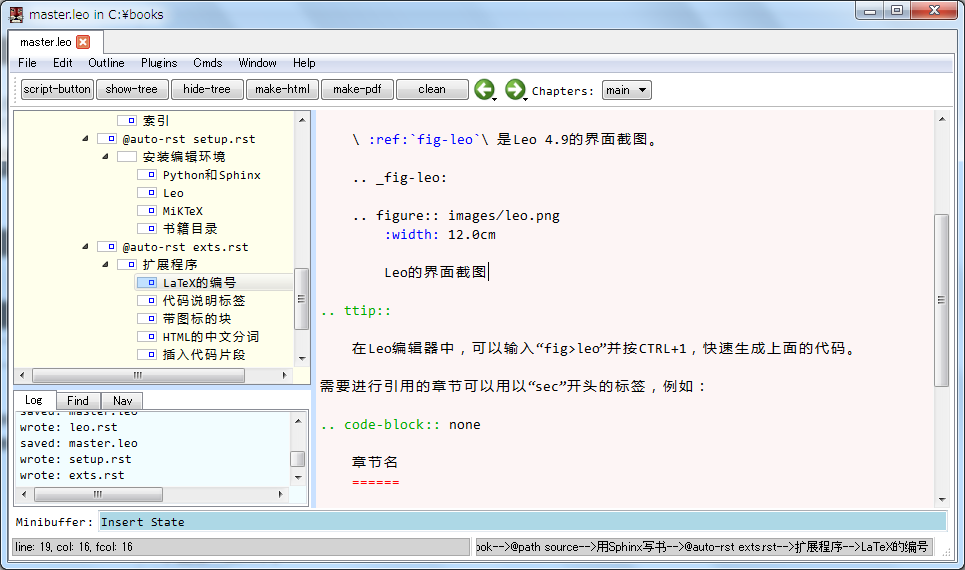
\includegraphics[width=12.0cm]{leo.png}
\caption{Leo的界面截图}\label{leo:fig-leo}\end{figure}


\section{按钮工具栏}
\label{leo:sec-leo-buttons}\label{leo:id1}\phantomsection\label{leo:-sec-leo-buttons}
打开“master.leo”之后,可以在窗口的上方看到如下图所示的按钮工具栏。


\begin{threeparttable}
\capstart\caption{Leo的按钮工具栏说明}

\begin{tabulary}{\linewidth}{|L|L|}
\hline
\textbf{
按钮名
} & \textbf{
功能
}\\\hline

script-button
 & 
Leo自带的按钮,用它可以创建新的按钮
\\\hline

show-tree
 & 
显示并调整提纲窗口的宽度
\\\hline

hide-tree
 & 
隐藏提纲窗口
\\\hline

make-html
 & 
将当前的书籍项目编译为HTML
\\\hline

make-pdf
 & 
将当前的书籍项目编译为PDF
\\\hline

clean
 & 
清除当前的书籍项目的编译结果
\\\hline
\end{tabulary}

\end{threeparttable}


其中,make-html、make-pdf以及clean等三个按钮,需要提纲栏中的当前节点为某个书籍项目的子节点。


\section{快速输入宏}
\label{leo:id2}
在“master.leo”中定义了可快速输入各种命令的宏,其节点路径为:

\begin{Verbatim}[commandchars=\\\{\}]
@chapters\PYGZhy{}\PYGZhy{}\PYGZgt{}Scripts\PYGZhy{}\PYGZhy{}\PYGZgt{}@command rst\PYGZhy{}macro
\end{Verbatim}

输入宏之后按CTRL+1即可执行,将其扩展为对应的文本。下表列出了一些常用的宏:


\begin{threeparttable}
\capstart\caption{快速输入文本的宏}

\begin{tabulary}{\linewidth}{|L|L|}
\hline
\textbf{
输入
} & \textbf{
输出
}\\\hline

table
 & 
table命令
\\\hline

inc\textgreater{}
 & 
literalinclude命令
\\\hline

math
 & 
math命令
\\\hline

fig\textgreater{}
 & 
figure命令
\\\hline

\_s
 & 
章节标签
\\\hline

\_f
 & 
图表标签
\\\hline

sec
 & 
章节参照
\\\hline

fig
 & 
图表参照
\\\hline

m
 & 
行内math命令
\\\hline

tl
 & 
tlink命令
\\\hline

tt
 & 
ttip命令
\\\hline

tw
 & 
twaring命令
\\\hline

tc
 & 
tcode命令
\\\hline

ta
 & 
tanim命令
\\\hline

cb
 & 
code-block命令
\\\hline

t
 & 
topic命令
\\\hline

l
 & 
超链接
\\\hline

数字
 & 
对应的符号,如{\Large\ding{202}}\hspace{1mm}
\\\hline

-\textgreater{}
 & 
\(\rightarrow\)
\\\hline
\end{tabulary}

\end{threeparttable}


其中带“\textgreater{}”的宏可以输入参数,例如“fig\textgreater{}leo.png”、“inc\textgreater{}example.py\textgreater{}1”等。


\chapter{解决方案}
\label{tips::doc}\label{tips:id1}
本章列出一些在写书过程中经常会遇到的问题。


\section{表格}
\label{tips:id2}

\begin{threeparttable}
\capstart\caption{Python中的常用类型}

\begin{tabulary}{\linewidth}{|L|L|L|}
\hline
\textbf{
类型
} & \textbf{
描述
} & \textbf{
例子
}\\\hline

str
 & 
一个由字符组成的不可更改的有串行。在Python 3.x里,字符串由Unicode字符组成。
 & 
`Wikipedia', ``Wikipedia''
\\\hline

bytes
 & 
一个由字节组成的不可更改的有串行。
 & 
b'Some ASCII', b''Some ASCII''
\\\hline

list
 & 
可以包含多种类型的可改变的有串行
 & 
{[}4.0, `string', True{]}
\\\hline

tuple
 & 
可以包含多种类型的不可改变的有串行
 & 
(4.0, `string', True)
\\\hline

set, frozenset
 & 
与数学中集合的概念类似。无序的、每个元素唯一。
 & 
\{4.0, `string', True\}, frozenset({[}4.0, `string', True{]})
\\\hline

dict
 & 
一个可改变的由键值对组成的无串行。
 & 
\{`key1': 1.0, 3: False\}
\\\hline

int
 & 
精度不限的整数
 & 
42
\\\hline

float
 & 
浮点数。精度与系统相关。
 & 
3.1415927
\\\hline

complex
 & 
复数
 & 
3+2.7j
\\\hline

bool
 & 
逻辑值。
 & 
只有两个值:True和False
\\\hline
\end{tabulary}

\end{threeparttable}



\section{插图}
\label{tips:sec-tips-figure}\label{tips:id3}\phantomsection\label{tips:-sec-tips-figure}
当图像文件名以''.*''结尾时,将根据输出格式自动选择图像文件。例如,{\hyperref[tips:fig-fftexamplerectangle]{图\ref*{tips:fig-fftexamplerectangle}}}采用的文件名为“.*”,它对应两个文件:“fft\_example\_rectangle.png”和“fft\_example\_rectangle.pdf”。输出HTML时将选用PNG文件,而输出PDF时将选用PDF文件。

\begin{Verbatim}[commandchars=\\\{\}]
.. figure:: images/fft\PYGZus{}example\PYGZus{}rectangle.*
\end{Verbatim}
\begin{figure}[htbp]
\centering
\capstart

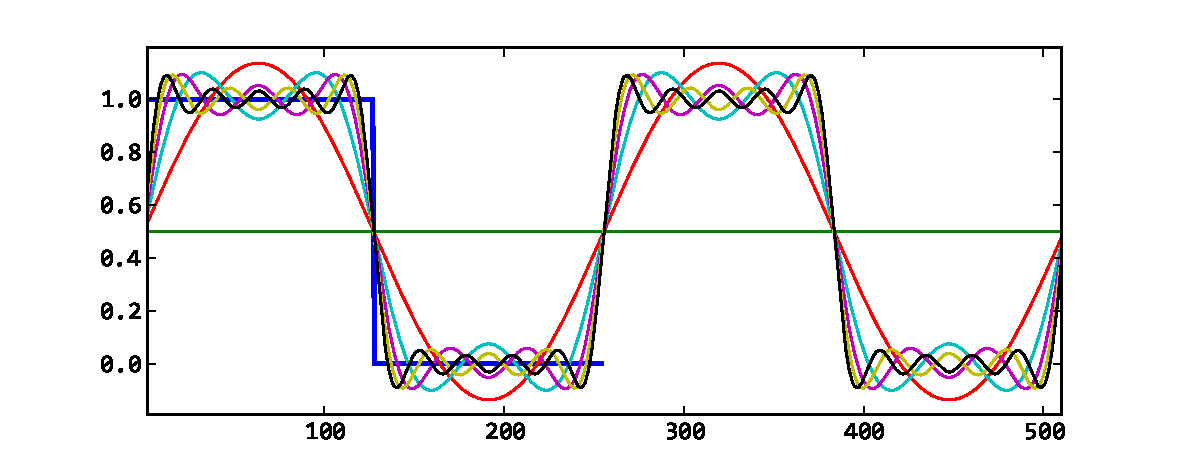
\includegraphics[width=14.0cm]{fft_example_rectangle.pdf}
\caption{用正弦波合成矩形波}\label{tips:fig-fftexamplerectangle}\end{figure}

{\hyperref[tips:fig-numpyaccess2d]{图\ref*{tips:fig-numpyaccess2d}}}采用的文件名为“numpy\_access2d.*”,对应两个文件:“numpy\_access2d.html.png”和“numpy\_access2d.latex.png”。

\begin{Verbatim}[commandchars=\\\{\}]
.. figure:: images/numpy\PYGZus{}access2d.*
\end{Verbatim}
\begin{figure}[htbp]
\centering
\capstart

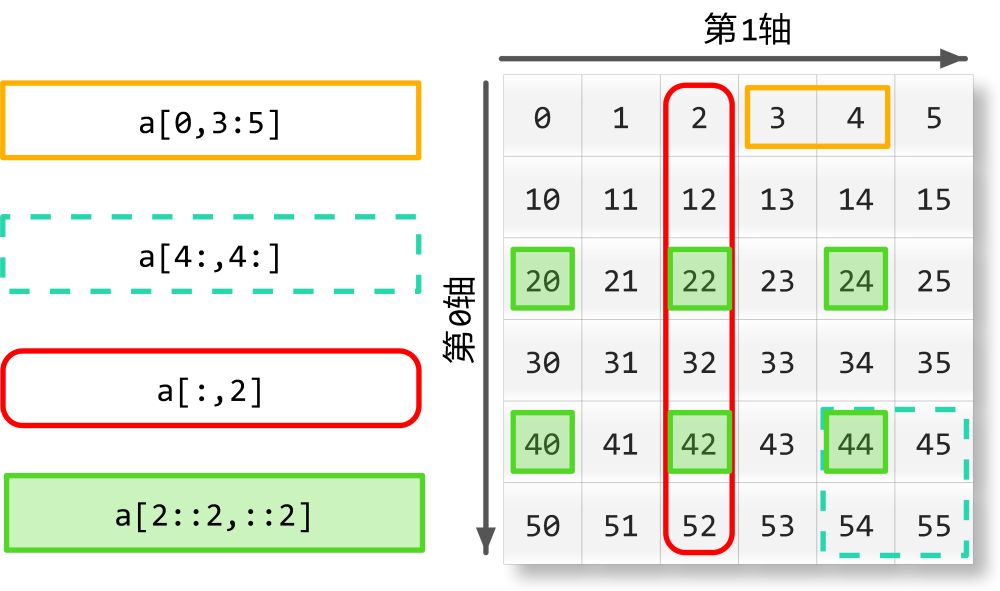
\includegraphics[width=12.0cm]{numpy_access2d.latex.png}
\caption{二维NumPy数组的下标存取}\label{tips:fig-numpyaccess2d}\end{figure}


\section{插入代码}
\label{tips:id4}
\begin{Verbatim}[commandchars=\\\{\},numbers=left,firstnumber=1,stepnumber=1]
\PYG{k}{class} \PYG{n+nc}{Directive}\PYG{p}{(}\PYG{n+nb}{object}\PYG{p}{)}\PYG{p}{:}
    \PYG{n}{Fake} \PYG{n}{Directive} \PYG{k}{class} \PYG{n+nc}{to} \PYG{n}{allow} \PYG{n}{Sphinx} \PYG{n}{directives} \PYG{n}{to} \PYG{n}{be} \PYG{n}{written} \PYG{o+ow}{in}
    \PYG{k}{class} \PYG{n+nc}{style}\PYG{o}{.}
    \PYG{l+s}{\PYGZdq{}\PYGZdq{}\PYGZdq{}}
\end{Verbatim}

\begin{Verbatim}[commandchars=\\\{\}]
\PYG{c}{\PYGZpc{}DOCLINK \PYGZhy{} Provide windows dir HREF text(clipboard)}

\PYG{n}{string\PYGZus{}temp\PYGZus{}ahead} \PYG{p}{=} \PYG{n}{fullfile}\PYG{p}{(}\PYG{l+s}{\PYGZsq{}}\PYG{l+s}{jar:file:///\PYGZsq{}}\PYG{p}{,} \PYG{n}{matlabroot}\PYG{p}{,} \PYG{l+s}{\PYGZsq{}}\PYG{l+s}{help\PYGZsq{}}\PYG{p}{)}\PYG{p}{;}

\PYG{n}{clipboard}\PYG{p}{(}\PYG{l+s}{\PYGZsq{}}\PYG{l+s}{copy\PYGZsq{}}\PYG{p}{,} \PYG{n}{href\PYGZus{}for\PYGZus{}codelib}\PYG{p}{)}\PYG{p}{;}
\end{Verbatim}


\chapter{索引}
\label{index:id1}\begin{itemize}
\item {} 
\emph{genindex}

\item {} 
\emph{search}

\end{itemize}



\renewcommand{\indexname}{索引}
\printindex
\end{document}
